\subsection{State (\textit{o Object for States})}
\label{state}

\textbf{Scopo}: Comportamentale \\
\textbf{Raggio d'azione}: Oggetti

\paragraph{Definizione} Il pattern State permette ad un oggetto di cambiare il suo comportamento al cambiare del suo stato interno. L'oggetto si comporterà come se avesse cambiato la sua classe, o meglio, cambia il modo con cui reagisce alla chiamata di un certo metodo.

Il comportamento dell'oggetto dipende dal proprio stato e deve cambiare durante l'esecuzione in funzione dello stato corrente.

Esistono metodi con grandi blocchi di codice per scelte condizionali il cui esito dipende dallo stato dell’oggetto. Di solito lo stato è rappresentato in questi casi da costanti. 

Il pattern State confina ogni ramo condizionale in una classe separata (per evitare di applicazioni azioni diverse con comandi quali switch).

\begin{figure}[H]
    \centering
    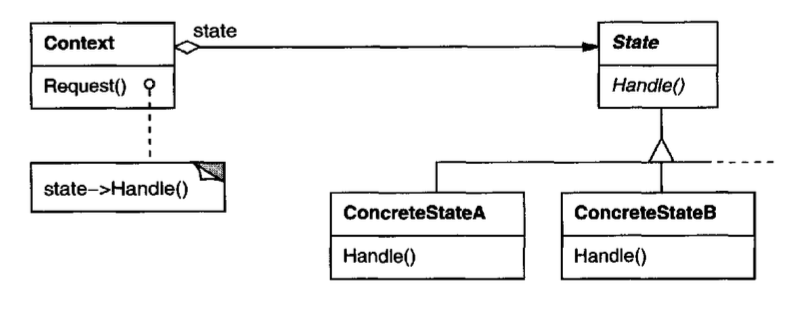
\includegraphics[width=1\linewidth]{assets/pattern/state/state-struttura.png}
    \caption{Struttura del pattern}
\end{figure}

\paragraph{Struttura e Conseguenze} Il pattern è composto da:
\begin{itemize}
    \item \textbf{Context}: definisce l’interfaccia utilizzata dai client. Mantiene un riferimento ad un’istanza di una classe che implementa l’interfaccia State e che rappresenta lo stato corrente. 
    \item \textbf{State}: Definisce un’interfaccia che incapsula il comportamento associato ad uno stato particolare di Context. 
    \item \textbf{ConcreteState}: Ogni classe che occupa questo ruolo definisce un particolare comportamento associato ad uno stato di Context.
\end{itemize}

Il pattern permette di localizzare il comportamento specifico di uno stato e suddividere il comportamento in funzione di esso, in più rende esplicite le transizioni di stato (atomiche dal p.d.v. di Context) ed è adatto alla condivisione.

È bene notare che l'applicazione del modello risulta eccessiva per applicazioni che presentano pochi stati o che cambiano raramente.

Può essere correlato ai pattern Flyweight (\ref{flyweight}, utilizzato per la condivisione di oggetti State) e Singleton (\ref{singleton}, spesso gli oggetti State sono dei Singleton)

\newpage